\addcontentsline{toc}{chapter}{Application Layer}
\chapter*{\begin{center}Application Layer\end{center}}
\begin{center}(Layer 5 nello stack TCP/IP)\end{center}\hrulefill \\
\hrulefill \\
\addcontentsline{toc}{section}{Introduzione}
\section*{Introduzione}
Ci sono 2 principali architetture in cui gli host si dividono:
\begin{itemize}
    \item Client-Server (e.g.: web server);
    \item Peer-to-Peer;
\end{itemize}

\noindent Network application: coppia di processi che si scambiano messaggi.\\

\begin{figure} [h]
    \centering
    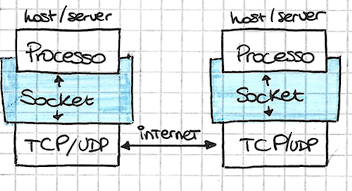
\includegraphics[width=0.5\linewidth]{Figures//02/netapps.png}
    \caption{Network application. Le \index{socket}socket (o API) sono interfacce software tra l'application layer e il transport layer di ciascun host. Ne esistono tra tutte le coppie di layer adiacenti.}
    \label{fig:enter-label}
\end{figure}

 \noindent Per identificare il processo ricevente serve specificare: l'indirizzo IP del Host, e un numero di porta\index{porta!numero di} che è dedicato al servizio (in maniera permanente o temporanea), tipo 100.100.100.1:80; ci sono diversi numeri di porta noti per essere riservati a certi servizi, tipo 80 è una porta riservata ad HTTP, 443 ad HTTPS, oppure 110 a POP3, 20 e 21 a FTP (dati e controllo rispettivamente), 67 e 68 a DHCP (requests e replies rispettivamente), 25 al mail server SMTP, 520 a RIP, e così via.\footnote{I numeri di porta sono documentati alla pagina: https://www.iana.org/assignments/service-names-port-numbers/service-names-port-numbers.xhtml}

\noindent La nostra app, a livello sottostante (transport layer), potrà usare principalmente due protocolli:
\begin{itemize}
    \item TCP (Transmission Control Protocol)\index{TCP}
    \begin{itemize}
        \item servizio orientato alla connessione (è richiesto che le parti comunicanti si identifichino e completino un handshake per iniziare a comunicare);
        \item trasferimento dati affidabile (gestione della perdita di pacchetti);
        \item HTTP, SMTP, FTP, HTTP 1.1, HTTPS, Telnet etc. si appoggiano tutti su TCP per il trasporto
    \end{itemize}
    \item UDP (User Datagram Protocol)\index{UDP}
    \begin{itemize}
        \item minimale, leggero, trasmette il minimo indispensabile delle informazioni necessarie per consegnare un pacchetto da punto A a punto B;
        \item connectionless: niente handshake, niente connessione preliminare tra A e B. Il messaggio viene sparato da A e se arriva o meno non è dato saperlo.
        \item per via della sua leggerezza, UDP alle volte viene utilizzato per lo streaming live e on-demand (e.g.: Twitch),  servizi per cui non è necessario garantire che tutti i dati arrivino a destinazione (al limite si perde qualche frame, ma il contenuto si capisce ancora abbastanza bene). 
    \end{itemize}
\end{itemize}

\begin{figure}[h]
    \centering
    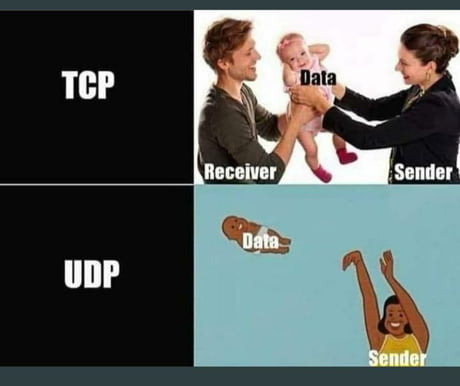
\includegraphics[width=0.5\linewidth]{Figures/02/tcp-udp.png}
    \caption{Non so a chi attribuire questa creazione, ma è uno dei miei esempi umoristici preferiti riguardo TCP vs UDP. Kudos al creatore originale.}
\end{figure}

\noindent Nessuno dei due implementa sistemi di crittografia, a meno che non si usi TCP con TLS (Transport Layer Security), ma di base TCP non fornisce questo servizio.\\

\addcontentsline{toc}{section}{HTTP}
\section*{\textcolor{RoyalBlue}{HTTP}} 
\index{HTTP}
\noindent \textcolor{RoyalBlue}{H}yper \textcolor{RoyalBlue}{T}ext \textcolor{RoyalBlue}{T}ransfer \textcolor{RoyalBlue}{P}rotocol, default port: 80\\

\noindent Protocollo a livello di applicazione \underline{Web}: una \index{web!pagina}pagina Web è un insieme di oggetti (e.g.: file HTML\footnote{Hyper Text Markup Language}, immagine JPEG, file JavaScript, file CSS...). Tipicamente alla base delle pagine Web c'è un file HTML di base, che fa riferimento agli altri oggetti della pagina attraverso i relativi \index{URL}URL\footnote{Uniform Resource Locator}.\\

\noindent I \index{web!browser}Web Browser (e.g.: Google Chrome) implementano il lato Client di HTTP;

\noindent È un protocollo stateless: se un client manda due richieste identiche nell'arco di qualche secondo, HTTP non ne ha alcuna memoria, risponderà 2 volte con la stessa risposta.

\noindent Connessioni TCP:
\begin{itemize}
    \item persistente: tutte le richieste/risposte avvengono nella stessa sessione TCP;
    \item non persistente: ogni richiesta/risposta avviene in una sessione TCP nuova a se stante (ogni volta ne viene avviata una nuova).
\end{itemize}
\noindent HTTP usa una connessione persistente di default, ma può usarle entrambe. \\

\noindent \index{round trip time}RTT - Round Trip Time: tempo impiegato da un pacchetto per andare da client a server e poi tornare indietro.

\begin{table}[h]
\centering
\begin{tabular}{|ll|}
\hline
\multicolumn{2}{|c|}{Messaggi HTTP} \\ \hline
\multicolumn{1}{|c|}{Richiesta} & \multicolumn{1}{c|}{Risposta}\\ \hline
\multicolumn{1}{|l|}{\begin{tabular}[c]{@{}l@{}}get$^1$ /dir/page.html$^2$ HTTP/1.1$^3$\\ $^1$Request line - metodo $^2$ URL $^3$ versione HTTP\end{tabular}}    & \begin{tabular}[c]{@{}l@{}}HTTP/1.1 200 OK$^4$\\ $^4$stato\end{tabular}            \\ \hline
\multicolumn{1}{|l|}{\begin{tabular}[c]{@{}l@{}}Header:\\ host: www.(...) \\ connection: close \textbackslash{}textit\{(non persistente)\}\\ user\_agent: Mozilla/5.0 (tipo browser)\\ ... *altre istruzioni HTTP*\end{tabular}} & \begin{tabular}[c]{@{}l@{}}Header:\\ connection: close\\ date:[current date]\\ server: Apache/2.2.3\\ last-modified: {[}date{]}\\ Content length: 6821 {[}byte{]}\\ Content type: text/html\\ *RIGA VUOTA, fine Header*\\ Contenuto: data data data...\end{tabular} \\ \hline
\end{tabular}
\end{table}

\noindent Qual è la differenza tra HTTP 1.0 e HTTP 1.1? La più importante forse è la persistenza della connessione (abbiamo visto cosa significa poco fa), oltre ad altre cose come, ad esempio, l'introduzione di meccaniche di caching.

\addcontentsline{toc}{subsection}{Cookies}
\subsection*{\textcolor{RawSienna}{Cookies}}
\index{cookies}


\noindent (argomento interno ad HTTP) I cookies sono un tipo di informazione che viene memorizzata lato client. Può servire in un secondo momento al server per ristabilire una connessione.

\begin{figure} [h]
    \centering
    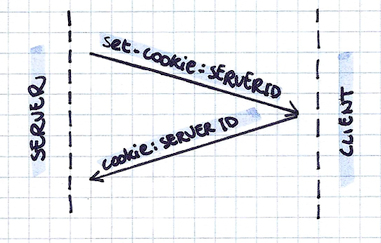
\includegraphics[width=0.6\linewidth]{Figures/02/cookies.png}
\end{figure}
\begin{itemize}
    \item ogni browser/sistema operativo archivia i cookies in un posto a sua discrezione, non esiste una convenzione universale su dove salvare i file di cookies;
    \item inizialmente, tutti i cookies erano semplici file di testo, ora la maggior parte è in formato SQLite (piccoli database!);
    \item non tutti i siti web usano i cookies;
    \item (tecnicamente,) i cookies sono \underline{facoltativi.}
    \item i cookies possono essere disabilitati;
    \item i cookies sono una minaccia per la privacy in quanto profilano gli utenti! Raccogliendo informazioni sulle loro abitudini, comportamenti etc. Vengono usati in quella che si dice Pubblicità comportamentale: analisi dell'attività in rete degli utenti al fine di permettere alle aziente di presentare a ciascuno pubblicità mirate ai loro gusti.\footnote{https://youronlinechoices.com/it/}
\end{itemize}


\addcontentsline{toc}{section}{Web Caching}
\section*{\textcolor{Brown}{Web Caching}}
\index{web!cache}\index{proxy server}
\noindent (o Proxy Server)\\

\noindent È un'entità della rete in grado di rispondere ad alcune richieste HTTP al posto dei server a cui sono indirizzate. Funziona circa così:
\begin{enumerate}
    \item Browser invia richiesta HTTP al proxy per (ad esempio) una pagina web;
    \item [2a] Se il Proxy contiene una copia in locale della pagina richiesta $\rightarrow$ il Proxy risponde al client;
    \item [2b] Se il Proxy non contiene una copia della pagina $\rightarrow$ il proxy richiede la pagina al server che dovrebbe averla, una volta che la ha ricevuta la recapita al client browser e ne salva una copia in locale. 
\end{enumerate}

\noindent ``Conditional GET'',\index{GET!conditional} richiesta dal proxy per il server: se l'oggetto richiesto è stato modificato di recente, mandamene la copia aggiornata, altrimenti manderò al client quella che ho io.\\

\noindent Perché si fa questo lavoro di web cache?
\begin{itemize}
    \item per ridurre i tempi di attesa\footnote{normalmente l'intensità di traffico è molto più alta al di fuori di una LAN (in uscita verso Internet) che non al suo interno, da cui le potenziali latenze elevate.};
    \item ridurre il traffico complessivo nel Web.
\end{itemize}
\noindent L'intensità del traffico\index{intensità di traffico} può essere misurata come: 
\[T = X \cdot \dfrac{Y}{Z}\]
dove:\\
$X=$ richieste/secondo;\\
$Y=$ Megabit/richiesta;\\
$Z=$ Megabit/secondo.\\


%%%%%%%%%%%%%%%%%%%%%%%%%%%%%%%%%%%%%%%%%%%%
%%%%%%%%%%%%%%%%%%%%%%%%%%%%%%%%%%%%%%%%%%%%

\addcontentsline{toc}{section}{Posta Elettronica}
\section*{\textcolor{Periwinkle}{e-Mail}}
\index{posta elettronica}
\noindent Componenti chiave del sistema di mailing in Internet:
\begin{itemize}
    \item User Agents\index{user agent}: lo strumento con cui si leggono/scrivono le mail, come la app di Gmail per Android o un browser web che accede al sito \hyperlink{mail.google.com}{https://mail.google.com/mail/};
    \item Mail Servers\index{mail!server}: il ``core'' dell'infrastruttura di e-mailing. È il mail server che contiene le caselle degli utenti, i messaggi viaggiano dal MS del mittente alla mailbox nel MS del destinatario/i;
    \item SMTP\index{SMTP} (Simple Mail Transfer Protocol): il principale protocollo a livello applicativo per la posta elettronica.
\end{itemize}

\noindent Principali comandi SMTP: HELO (hello), MAIL FROM, RCPT TO, DATA, QUIT. \\

\noindent SMPT è un ``push protocol'', si può usare solo per \textit{inviare} messaggi di posta elettronica; per richiedere dei messaggi da leggere, invece, occorre utilizzare un altro tipo di protocollo.\\

\noindent HTTP e IMAP (Internet Mail Access Protocol) permettono di fare cose come gestire cartelle, eliminare messaggi etc. Nello specifico, HTTP serve giusto a supporto di Web app come Gmail, IMAP in sé è sufficiente se si vuole richiedere un messaggio di posta da un server e leggerlo da un'interfaccia anche spartana.

\addcontentsline{toc}{subsection}{POP3}
\subsection*{\textcolor{Aquamarine}{POP3}}
\index{POP3}
\noindent POP3 è un protocollo di posta elettronica (\textcolor{Aquamarine}{P}ost \textcolor{Aquamarine}{O}ffice \textcolor{Aquamarine}{P}rotocol). Come IMAP, POP lavora in ASCII su 2 porte con TCP (110, 995). Comandi client per autenticazione sono semplicemente \texttt{user} e \texttt{pass}, il server risponde con \texttt{+ok} o \texttt{-err}.

\noindent Transazioni:
\begin{itemize}
    \item \texttt{list}: elenca i messaggi (numero e dimensione);
    \item \texttt{retr} $<n>$: retrive msg con numero $n$;
    \item \texttt{dele}: delete msg;
    \item \texttt{quit}: esci
\end{itemize}


\addcontentsline{toc}{section}{DNS}
\section*{\textcolor{OliveGreen}{DNS}}
\index{DNS}

\noindent \textcolor{OliveGreen}{D}omain \textcolor{OliveGreen}{N}ame \textcolor{OliveGreen}{S}ystem, default port: 53\\

\begin{wrapfigure}{r}{0.6\textwidth}
 \begin{center}
 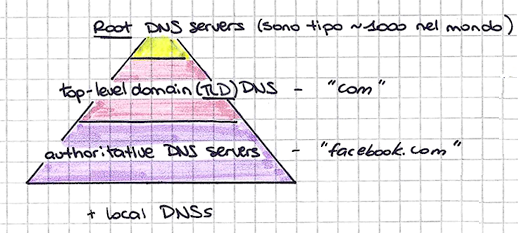
\includegraphics[width=1\linewidth]{Figures/02/dns-hiera.png}
  \end{center}
  \label{fig:gerarchia}
  \caption{Gerarchia a tre livelli dei DNS.}
\end{wrapfigure}

\noindent Si tratta di un database distribuito e di un protocollo a livello applicazione per inviare queries ai Server DNS, si occupa di \underline{tradurre} gli hostname\index{hostname} (e.g.: \textit{www.facebook.com}) nei corrispondenti indirizzi IP (e.g.: \textit{69.63.176.13}).\\

\noindent DNS offre servizi quali Host aliasing\index{host!aliasing} (tradurre un hostname in un altro hostname, spesso meno user-friendly di quello ricevuto), mail server aliasing, load distribution.\\

\noindent DNS Caching: stesso meccanismo del Web caching, ma applicato al DNS.\\

\noindent Resource Records (RR): informazioni immagazzinate nei database DNS. Sono triple della forma
\begin{verbatim}
    (Name, Value, Type, TTL)
\end{verbatim}
\noindent Dove TTL sta per Time-To-Live, tempo di vita del record nel database (scaduto il quale questo viene eliminato).

\begin{table}[h]
\begin{tabular}{|c|c|c|}
\hline
\textbf{Type} & \textbf{Name} & \textbf{Value}                                                \\ \hline
A             & hostname      & IP Address                                                    \\ \hline
NS           & domain        & hostname del DNS che sa ottenere l'IP degli host nel dominio  \\ \hline
CNAME         & host          & valore canonico per l'host che ha sinonimo *nome*             \\ \hline
MX            & host          & valore canonico di un mail server per host sinonimo di *nome* \\ \hline
\end{tabular}
\label{tab:rr}
\caption{Alcuni esempi di Resource Record. I valori dei campi ``Name'' e ``Value'' dipendono dal valore in ``Type''.}
\end{table}\index{resource record}

\addcontentsline{toc}{section}{Telnet}
\section*{\textcolor{RubineRed}{Telnet}}
\index{telnet}
\noindent Uno dei primi protocolli in assoluto per TCP/IP, basato su architettura client-server, molto semplice ma nella sua semplicità è deprecato, ora al suo posto si usa SSH (Secure SHell)\index{SSH}. Fondamentalmente Telnet permette di fare collegamenti ad altri terminali attraverso la rete (alla porta 23).\\

\noindent Come funziona: il client manda richieste al server Telnet, e quello risponde. Ogni tasto che viene battuto sulla tastiera del lato client, ogni singolo carattere, viene spedito sulla rete e ricevuto dal server. Il server, ricevuto un carattere, lo rimanda in risposta come una ``echo''. Quindi non stiamo parlando di digitare una parola o una frase e poi premere ``invio'' per inviarla al server, l'invio avviene lettera per lettera.\\Serve a fare accesso remoto ad altre macchine. Perché non si usa più e piuttosto si usa SSH? Perché Telnet trasmette in cleartext, ovvero: ogni carattere viene trasmesso in chiaro, senza essere cifrato in nessuna maniera. Attraversa la rete esattamente come viene scritto. Chiunque riesca a posizionarsi tra client e server potrebbe origliare ciò che viene detto e impossessarsi delle informazioni.

\addcontentsline{toc}{section}{Macchine Virtuali}
\section*{\textcolor{RedViolet}{Virtual Machines}}
\index{macchina virtuale}
\noindent (cenni).\\

\noindent Una Macchina Virtuale (VM), essenzialmente, è un software che, montato e avviato, è in grado di simulare un computer a sé stante istanziato all'interno del nostro computer. Virtualmente, è come se ritagliassimo qualche pezzetto hardware dal nostro computer e usassimo questi pezzetti per creare un computerino fatto dai ritagli del nostro computer. Ok, questo, ma a livello software. Senza segare letteralmente la CPU a metà.\\

\noindent Per fare ciò, presa un'immagine di un sistema operativo, dovremo usare un Hypervisor\index{hypervisor}, cioè un programma che virtualizza degli host usando l'hardware della nostra macchina. Se avete abbastanza risorse hardware, potreste anche avviare più di una macchina virtuale contemporaneamente! L'hypervisor che ci è stato consigliato si chiama \textbf{VirtualBox}\index{VirtualBox} di Oracle\footnote{https://www.virtualbox.org/wiki/Downloads}, in alternativa ce ne sono altre come VMWare Workstation\index{VMWare Workstation}. Perlomeno nelle versioni base, entrambi quelli che ho menzionato sono gratuiti.

\addcontentsline{toc}{section}{FTP}
\section*{\textcolor{Sepia}{FTP}}
\index{FTP}
\noindent \textcolor{Sepia}{F}ile \textcolor{Sepia}{T}ransfer \textcolor{Sepia}{P}rotocol. Protocollo per il trasferimento di files.\\

\begin{itemize}
    \item di tipo client-server;
    \item usa connessioni TCP su porte 20 e 21, entrambe aperte dal client:
    \begin{itemize}
        \item porta 20 per i dati;
        \item porta 21 per i comandi (controllo);
    \end{itemize}
    \item permette operazioni di upload e download;
    \item spesso oggi anziché usare FTP si preferisce scambiarsi file usando HTTP, perché come Telnet, anche in FTP tutte le informazioni transitano in chiaro, in formato ASCII.
\end{itemize}

\noindent Qualche comando FTP:
\begin{itemize}
    \item USER: username;
    \item PASS: password;
    \item LIST: elenca i contenuti della cartella;
    \item RETR: retrieve, richiedi un file;
    \item STORE: carica un file.
\end{itemize}

\noindent Come HTTP, FTP ha dei codici di stato (tipo il ``404 Not Found''). Alcuni codici sono:

\begin{itemize}
    \item 331 : username ok, password required;
    \item 125 : data connection already open; transfer starting;
    \item 425 : can't open data connection;
    \item 452 : error writing file;
\end{itemize}

\noindent Nel 99\% dei casi, FTP si usa da interfaccia a linea di comando (CLI): per avviare una connessione ftp, si usa il comando (è possibile autenticarsi anche come \texttt{anonymous})
\begin{verbatim}
    ftp <indirizzo>
\end{verbatim}

\noindent La questione PASV/PORT che forse vi interessa: in Windows 10, usare FTP può dare problemi a causa della questione della \textit{``modalità passiva/modalità port'' (PASV/PORT)}. PASV e PORT sono entrambi comandi per la connessione dati (una delle due porte usate da FTP, no? Dati e comandi, ecco, quella dei dati); la connessione dati FTP, a volte, viene ostacolata dai Firewall, quindi se in principio bastava usare il comando PORT, successivamente all'avvento di NAT e Firewall si è reso necessario aggiungere PASV, che non è altro che una modalità trasferimento dati compatibile con Firewall.

\addcontentsline{toc}{subsection}{tFTP}
\subsection*{\textcolor{Maroon}{tFTP}}
\index{tFTP}
\noindent Ovvero, \textcolor{Maroon}{t}rivial \textcolor{Maroon}{FTP}. A differenza di FTP, tFTP:
\begin{itemize}
    \item usa UDP (alla porta 69);
    \item ha pochissime funzioni (da cui il termine \textit{``trivial'', banale});
    \item non conosce il concetto di Directory (cartella);
    \item non usa autenticazione;
    \item ha quindi un utilizzo molto limitato;
    \item ha 2 modalità di trasferimento: ASCII (NETASCII) e binario (OCTET);
\end{itemize}

\noindent alcuni comandi tFTP:

\begin{itemize}
    \item \textbf{RR}: read request;
    \item \textbf{WR}: write request;
    \item \textbf{DATA}: dati;
    \item \textbf{ACK}: acknowledged;
    \item \textbf{ERR}: errore;
\end{itemize}

\noindent I pacchetti UDP inviati da tFTP sono a lunghezza fissa $= 512$ Bytes. La trasmissione si considera conclusa quando viene ricevuto un pacchetto di dimensioni $< 512$ B.

\addcontentsline{toc}{section}{SNMP}
\section*{\textcolor{WildStrawberry}{SNMP}}
\index{SNMP}
\noindent \textcolor{WildStrawberry}{S}imple \textcolor{WildStrawberry}{N}etwork \textcolor{WildStrawberry}{M}anagement \textcolor{WildStrawberry}{P}rotocol\\

\noindent Normalmente, se presente, la porta standard usata è 161 (UDP). Anche SNMP viene spesso bloccato dal firewall - com'è giusto che sia, visto che per design questo protocollo dovrebbe arrivare soltanto dall'interno.\\

\noindent Usato per gestione di reti, monitoraggio e configurazione di dispositivi di rete.\\

\noindent Consiste in un protocollo molto semplice che fa:
\begin{verbatim}
    GET - GETNEXT - GETBULK - SET - TRAP
\end{verbatim}

\noindent Fa uso di Access Control List (ACL)\index{access control list}, regole che indicano cosa può e cosa non può fare un dispositivo);\\

\noindent Si possono istanziare manager o agent ($\approx$ server, cioè un'entità che ha il suo database di MIB, Management Info Base) - ogni oggetto MIB è identificato da una serie di numeri in un formato tipo:
\begin{verbatim}
    1.3.6.1.2.1.1.3 = SysUptime
\end{verbatim}

\noindent E' un modo macchinoso di immagazzinare informazioni riguardo il device e la rete. Tutti quei numeretti sono come un sistema di coordinate GPS, l'interno di questi record somiglia vagamente a un JSON.
\newpage